\documentclass[letterpaper]{article}
\usepackage[margin=1in]{geometry}
\usepackage[utf8]{inputenc}
\usepackage{textcomp}
\usepackage{amssymb}
\usepackage{natbib}
\usepackage{graphicx}
\usepackage{gensymb}
\usepackage{amsthm, amsmath, mathtools}
\usepackage[dvipsnames]{xcolor}
\usepackage{enumerate}
\usepackage{mdframed}
\usepackage[most]{tcolorbox}
\usepackage{csquotes}
% https://tex.stackexchange.com/questions/13506/how-to-continue-the-framed-text-box-on-multiple-pages

\tcbuselibrary{theorems}

\newcommand{\R}{\mathbb{R}}
\newcommand{\Z}{\mathbb{Z}}
\newcommand{\N}{\mathbb{N}}
\newcommand{\Q}{\mathbb{Q}}
\newcommand{\C}{\mathbb{C}}
\newcommand{\code}[1]{\texttt{#1}}
\newcommand{\mdiamond}{$\diamondsuit$}
\newcommand{\PowerSet}{\mathcal{P}}
\newcommand{\Mod}[1]{\ (\mathrm{mod}\ #1)}
\DeclareMathOperator{\lcm}{lcm}

%\newtheorem*{theorem}{Theorem}
%\newtheorem*{definition}{Definition}
%\newtheorem*{corollary}{Corollary}
%\newtheorem*{lemma}{Lemma}
\newtheorem*{proposition}{Proposition}


\newtcbtheorem[number within=section]{theorem}{Theorem}
{colback=green!5,colframe=green!35!black,fonttitle=\bfseries}{th}

\newtcbtheorem[number within=section]{definition}{Definition}
{colback=blue!5,colframe=blue!35!black,fonttitle=\bfseries}{def}

\newtcbtheorem[number within=section]{corollary}{Corollary}
{colback=yellow!5,colframe=yellow!35!black,fonttitle=\bfseries}{cor}

\newtcbtheorem[number within=section]{lemma}{Lemma}
{colback=red!5,colframe=red!35!black,fonttitle=\bfseries}{lem}

\newtcbtheorem[number within=section]{example}{Example}
{colback=white!5,colframe=white!35!black,fonttitle=\bfseries}{def}

\newtcbtheorem[number within=section]{note}{Important Note}{
        enhanced,
        sharp corners,
        attach boxed title to top left={
            xshift=-1mm,
            yshift=-5mm,
            yshifttext=-1mm
        },
        top=1.5em,
        colback=white,
        colframe=black,
        fonttitle=\bfseries,
        boxed title style={
            sharp corners,
            size=small,
            colback=red!75!black,
            colframe=red!75!black,
        } 
    }{impnote}
\usepackage[utf8]{inputenc}
\usepackage[english]{babel}
\usepackage{fancyhdr}
\usepackage[hidelinks]{hyperref}

\pagestyle{fancy}
\fancyhf{}
\rhead{Math 170B}
\chead{Monday, May 01, 2023}
\lhead{Lecture 13}
\rfoot{\thepage}

\setlength{\parindent}{0pt}

\begin{document}

\section{Spline lnterpolation (Section 6.4)}
A \textbf{spline function} consists of polynomial pieces on subintervals joined together with certain continuity conditions. Formally, suppose we have $m + 1$ \textbf{ordered} points, called \textbf{knots}, $t_0, t_1, \hdots, t_m$ (i.e., we know the values of each $t_i$ and $t_i < t_{i + 1}$). Thus, a \textbf{spline function of degree} $k$ having knots $t_0, t_1, \hdots, t_m$ is a function $S$ such that 
\begin{enumerate}
    \item On each interval $[t_{i - 1}, t_i)$, $S$ is a polynomial of degree $\leq k$.
    \item On $[t_0, t_n]$, $S$ has a continuous $(k - 1)$th derivative.
\end{enumerate}
Basically, $S$ is a piecewise polynomial of degree at most $k$ having continuous derivatives of all orders up to $k - 1$. 

\subsection{Degree 1 Spline Functions}
Let $k = 1$ so that we have a degree one spline function. Suppose we have coefficients $a_i, b_i$. Then, we can define the spline function $S$ as 
\[S = \begin{cases}
    S_{0}(x) = a_0 x + b_0 & x \in [t_0, t_1) \\ 
    S_{1}(x) = a_1 x + b_1 & x \in [t_1, t_2) \\ 
    \vdots \\ 
    S_{m - 1}(x) = a_{m - 1}x + b_{m - 1} & x \in [t_{m - 1}, t]
\end{cases}.\]
From the second property, $S(x)$ is continuous, so the piecewise polynomials match up at the nodes. That is, $\boxed{S_{i}(t_{i + 1}) = S_{i + 1}(t_{i + 1}).}$
\begin{center}
    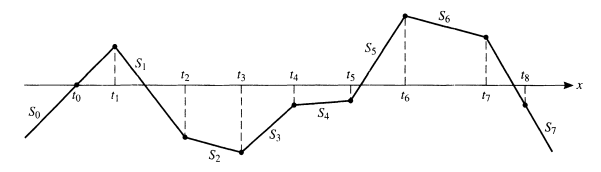
\includegraphics[scale=0.6]{../assets/spline.png}
\end{center}
\textbf{Remark:} This typically extends the knots. In other words, we might see 
\[S = \begin{cases}
    S_{0}(x) & x \in (-\infty, t_1] \\ 
    S_{m - 1}(x) & x \in [t_{m - 1}, \infty)
\end{cases}.\]

\subsubsection{Algorithm for Degree 1 Spline Functions}
We can write some code to evaluate a \textbf{degree 1 spline}. The inputs are the coefficients $\{a_i\}$, $\{b_i\}$, the knot values $\{t_j\}$, and $x$ such that $0 \leq i \leq m - 1$ and $0 \leq j \leq m$. 
\begin{algorithm}[H]
    \caption{Degree 1 Spline}
    \label{alg:one}
    \begin{algorithmic}[1]
        \Function{DegOneSpline}{$\{a_i\}, \{b_i\}, \{t_j\}, x$}
            \State $s \gets a_{m - 1} x + b_{m - 1}$
            \For{$i \gets 1$ to $m - 1$}
                \If{$x \leq t_i$}
                    \State $s \gets a_{i - 1} x + b_{i - 1}$ \Comment{Search into which interval $x$ falls into.}
                    \State \textbf{break}
                \EndIf 
            \EndFor 
        \EndFunction
    \end{algorithmic}
\end{algorithm}

\subsection{Cubic Spline Functions}
We will now consider spline functions of degree 3, i.e., $k = 3$. Given the data points 
\begin{center}
    \begin{tabular}{c|c c c c c}
        $x$ & $t_1$ & $t_2$ & $t_3$ & $\hdots$ & $t_m$ \\
        \hline  
        $y$ & $y_1$ & $y_2$ & $y_3$ & $\hdots$ & $y_m$
    \end{tabular}
\end{center}
we want to construct an interpolating cubic spline,
\[S(x) = \begin{cases}
    S_{0}(x) & x \in [t_0, t_1] \\ 
    S_{1}(x) & x \in [t_1, t_2] \\ 
    S_{2}(x) & x \in [t_2, t_3] \\ 
    \vdots \\ 
    S_{m - 1}(x) & x \in [t_{m - 1}, t_m]
\end{cases}.\]
Each piece of $S(x)$ will be cubic polynomials. There are $4m$ unknown coefficients\footnote{Recall that a cubic function looks like $ax^3 + bx^2 + cx + d$, with four coefficients.}. 

\subsubsection{Evaluation Conditions}
The conditions for evaluating degree 3 polynomials are conditions for interpolation and continuity.
\begin{itemize}
    \item Interpolation: for $0 \leq i \leq m - 1$, we have  
    \[S_{i}(t_i) = y_i\]
    \[S_{i}(t_{i + 1}) = y_{i + 1}.\]
    There are a total of $2m$ conditions here. 

    \item Continuity: for $0 \leq i \leq m - 2$, we have 
    \[S_{i}'(t_{i + 1}) = S_{i + 1}'(t_{i + 1})\]
    \[S_{i}''(t_{i + 1}) = S_{i + 1}''(t_{i + 1})\]
    There are $2(m - 1)$ conditions here.
\end{itemize}
In total, there are $2m + 2(m - 1)$ conditions. 

\subsubsection{Finding \texorpdfstring{$S(x)$}{S(x)}}

Define the coefficients as $z_i = S_{i}''(t_i)$ for $1 \leq i \leq m - 1$. We know that $S_{i}''(x)$ is a linear function\footnote{Since it's the \emph{second} derivative of a cubic function.} on $[t_i, t_{i + 1}]$. Hence, we can write 
\[S_{i}''(x) = z_i \frac{(x - t_{i + 1})}{(t_i - t_{i + 1})} + z_{i + 1}\frac{(x - t_i)}{(t_{i + 1} - t_i)}.\]
Then, 
\[S_{i}''(t_i) = z_i \frac{(t_i - t_{i + 1})}{(t_i - t_{i + 1})} + z_{i + 1}\frac{(t_i - t_i)}{(t_{i + 1} - t_i)} = z_i.\]
Let $h_i = t_{i + 1} - t_i$. Then,
\[S_{i}''(x) = -\frac{z_i}{h_i}(x - t_{i + 1}) + \frac{z_{i + 1}}{h_i}(x - t_i)\]
Integrating yields
\[S_{i}'(x) = -\frac{z_i}{2z_i}(x - t_{i + 1})^2 + \frac{z_{i + 1}}{2h_i}(x - t_i)^2 + C,\]
where $C$ is an arbitrary constants. Integrating again yields  
\[S_i (x) = -\frac{z_i}{6h_i}(x - t_{i + 1})^3 + \frac{z_{i + 1}}{6h_i} (x - t_i)^3 + Cx + D\]
for some arbitrary $D$. For easier computation, we can write 
\[A_1 x + A_2 = C(x - t_i) + D(t_{i + 1} - x)\]
for some arbitrary $A_1, A_2, C, D$. Then, 
\[S_{i}(x) = -\frac{z_i}{6h_i}(x - t_{i + 1})^3 + \frac{z_{i + 1}}{6h_i} (x - t_i)^3 + C(x - t_i) + D(t_{i + 1} - x).\]



\end{document}